%% Преамбула TeX-файла

% 1. Стиль и язык
 \documentclass[utf8x, 14pt]{G7-32}

% \newfontfamily{\FA}{[FontAwesome.otf]}
% \usepackage{graphicx}
% \documentclass[utf8x, times, 14pt]{G7-32}

%% Стиль (по умолчанию будет 14pt)

% Остальные стандартные настройки убраны в preamble.inc.tex.
\sloppy
% Настройки стиля ГОСТ 7-32
% Для начала определяем, хотим мы или нет, чтобы рисунки и таблицы нумеровались в пределах раздела, или нам нужна сквозная нумерация.
\EqInChapter % формулы будут нумероваться в пределах раздела
\TableInChapter % таблицы будут нумероваться в пределах раздела
\PicInChapter % рисунки будут нумероваться в пределах раздела

% Добавляем гипертекстовое оглавление в PDF
\usepackage[
bookmarks=true, colorlinks=true, unicode=true,
urlcolor=black,linkcolor=black, anchorcolor=black,
citecolor=black, menucolor=black, filecolor=black,
]{hyperref}

\AfterHyperrefFix

% добавил для оформления алгоритмов
% вариант 1
%\usepackage{algorithm2e}
% вариант 2
\usepackage{algorithm}
\usepackage{algpseudocode}
% для таблиц
\usepackage{ctable}% http://ctan.org/pkg/ctable
\usepackage{caption}% http://ctan.org/pkg/caption



\usepackage{microtype}% полезный пакет для микротипографии, увы под xelatex мало чего умеет, но под pdflatex хорошо улучшает читаемость

% Тире могут быть невидимы в Adobe Reader
\ifInvisibleDashes
\MakeDashesBold
\fi

\usepackage{graphicx}   % Пакет для включения рисунков

% С такими оно полями оно работает по-умолчанию:
% \RequirePackage[left=20mm,right=10mm,top=20mm,bottom=20mm,headsep=0pt,includefoot]{geometry}
% Если вас тошнит от поля в 10мм --- увеличивайте до 20-ти, ну и про переплёт не забывайте:
\geometry{right=20mm}
\geometry{left=30mm}
\geometry{bottom=20mm}
\geometry{ignorefoot}% считать от нижней границы текста


% Пакет Tikz
\usepackage{tikz}
\usetikzlibrary{arrows,positioning,shadows}

% Произвольная нумерация списков.
\usepackage{enumerate}

% ячейки в несколько строчек
\usepackage{multirow}

% itemize внутри tabular
\usepackage{paralist,array}

%\setlength{\parskip}{1ex plus0.5ex minus0.5ex} % разрыв между абзацами
\setlength{\parskip}{1ex} % разрыв между абзацами
\usepackage{blindtext}

% Центрирование подписей к плавающим окружениям
%\usepackage[justification=centering]{caption}

\usepackage{newfloat}
\DeclareFloatingEnvironment[
placement={!ht},
name=Equation
]{eqndescNoIndent}
\edef\fixEqndesc{\noexpand\setlength{\noexpand\parindent}{\the\parindent}\noexpand\setlength{\noexpand\parskip}{\the\parskip}}
\newenvironment{eqndesc}[1][!ht]{%
    \begin{eqndescNoIndent}[#1]%
\fixEqndesc%
}
{\end{eqndescNoIndent}}




% Настройки листингов.
\ifPDFTeX
% 8 Листинги

\usepackage{listings}

% Значения по умолчанию
\lstset{
  basicstyle= \footnotesize,
  breakatwhitespace=true,% разрыв строк только на whitespacce
  breaklines=true,       % переносить длинные строки
%   captionpos=b,          % подписи снизу -- вроде не надо
  inputencoding=koi8-r,
  numbers=left,          % нумерация слева
  numberstyle=\footnotesize,
  showspaces=false,      % показывать пробелы подчеркиваниями -- идиотизм 70-х годов
  showstringspaces=false,
  showtabs=false,        % и табы тоже
  stepnumber=1,
  tabsize=4,              % кому нужны табы по 8 символов?
  frame=single
}

% Стиль для псевдокода: строчки обычно короткие, поэтому размер шрифта побольше
\lstdefinestyle{pseudocode}{
  basicstyle=\small,
  keywordstyle=\color{black}\bfseries\underbar,
  language=Pseudocode,
  numberstyle=\footnotesize,
  commentstyle=\footnotesize\it
}

% Стиль для обычного кода: маленький шрифт
\lstdefinestyle{realcode}{
  basicstyle=\scriptsize,
  numberstyle=\footnotesize
}

% Стиль для коротких кусков обычного кода: средний шрифт
\lstdefinestyle{simplecode}{
  basicstyle=\footnotesize,
  numberstyle=\footnotesize
}

% Стиль для BNF
\lstdefinestyle{grammar}{
  basicstyle=\footnotesize,
  numberstyle=\footnotesize,
  stringstyle=\bfseries\ttfamily,
  language=BNF
}

% Определим свой язык для написания псевдокодов на основе Python
\lstdefinelanguage[]{Pseudocode}[]{Python}{
  morekeywords={each,empty,wait,do},% ключевые слова добавлять сюда
  morecomment=[s]{\{}{\}},% комменты {а-ля Pascal} смотрятся нагляднее
  literate=% а сюда добавлять операторы, которые хотите отображать как мат. символы
    {->}{\ensuremath{$\rightarrow$}~}2%
    {<-}{\ensuremath{$\leftarrow$}~}2%
    {:=}{\ensuremath{$\leftarrow$}~}2%
    {<--}{\ensuremath{$\Longleftarrow$}~}2%
}[keywords,comments]

% Свой язык для задания грамматик в BNF
\lstdefinelanguage[]{BNF}[]{}{
  morekeywords={},
  morecomment=[s]{@}{@},
  morestring=[b]",%
  literate=%
    {->}{\ensuremath{$\rightarrow$}~}2%
    {*}{\ensuremath{$^*$}~}2%
    {+}{\ensuremath{$^+$}~}2%
    {|}{\ensuremath{$|$}~}2%
}[keywords,comments,strings]

% Подписи к листингам на русском языке.
\renewcommand\lstlistingname{Листинг}
\renewcommand\lstlistlistingname{Листинги}

\else
\usepackage{local-minted}
\fi

% Полезные макросы листингов.
% Любимые команды
\newcommand{\Code}[1]{\textbf{#1}}


% Стиль титульного листа и заголовки
% \include{00-title}


\begin{document}

\frontmatter % выключает нумерацию ВСЕГО; здесь начинаются ненумерованные главы: реферат, введение, глоссарий, сокращения и прочее.

% \maketitle %создает титульную страницу


% \begin{executors}
% \personalSignature{Первый исполнитель}{ФИО}

% \personalSignature{Второй исполнитель}{ФИО}
% \end{executors}


%\listoffigures                         % Список рисунков

%\listoftables                          % Список таблиц

%\NormRefs % Нормативные ссылки 
% Команды \breakingbeforechapters и \nonbreakingbeforechapters
% управляют разрывом страницы перед главами.
% По-умолчанию страница разрывается.

% \nobreakingbeforechapters
% \breakingbeforechapters

% \include{00-abstract}

\tableofcontents

\printnomenclature % Автоматический список сокращений

% \include{12-intro}

\mainmatter % это включает нумерацию глав и секций в документе ниже

\setcounter{page}{2}

\chapter{XFEM}
\label{cha:analysis}
\section{Постановка задачи}
В области $\Omega$ заданы уравнения равновесия \cite{Pisarenko1981}
\begin{equation}
%\sum\limits_{j=1}^{3} \frac{\partial\sigma_{ij}}{\partial x_j} = 0, i=\overline{1,3}.
%\frac{\partial\sigma_{ij}}{\partial x_j} = 0, i=\overline{1,3}.
%\bigtriangledown_j\sigma_{ij} = 0.%, i=\overline{1,3}.
\frac{\partial\sigma_{ij}}{\partial x_j} = 0.%, i=\overline{1,3}.
\label{F:F1}
\end{equation}
На границе $S=S_{1}\cup S_{2}$ заданы кинематические и силовые
краевые условия
\begin{equation}
\left.\mathbf{u}\right|_{S_{1}}=\mathbf{u}_{0}\left(t\right),
\label{F:F2}
\end{equation}
\begin{equation}
%\left.\sum\limits_{j=1}^{3}\sigma_{ij}n_j\right|_{S_{2}}=P_{i}\left(t\right),\:i=\overline{1,3},
\left.\sigma_{ij}n_j\right|_{S_{2}}=P_{i}\left(t,\,\mathbf{u}\right),% i=\overline{1,3},
\label{F:F3}
\end{equation}
где $\mathbf{u}$ --- вектор перемещения, $\mathbf{n}$ --- внешняя единичная нормаль к поверхности $S_{2}$, $\mathbf{P}$ --- вектор поверхностных сил.

Компоненты тензора малых деформаций Коши $\varepsilon$ связаны с перемещениями линейными геометрическими соотношениями
\begin{equation}
\varepsilon_{ij}=\frac{1}{2} \left(\frac{\partial u_{i}}{\partial x_{j}} + \frac{\partial u_{j}}{\partial x_{i}} \right).
\label{F:F4}
\end{equation}

Для изотропного тела тензор напряжений Коши $\sigma$ выражается через упругую составляющую $\varepsilon^{e}$ малой деформации Коши обобщенным законом Гука
\begin{equation}
%\sigma_{ij}=\sum\limits_{l=1}^{3} \sum\limits_{k=1}^{3} C_{ijkl}\varepsilon_{kl}^{e},
%\sigma_{ij}=C_{ijkl}\varepsilon_{kl}^{e},
\sigma=C:\varepsilon^{e},
\label{F:F_Hook}
\end{equation}
\begin{equation}
C_{ijkl}=\lambda\delta_{ij}\delta_{kl}+\mu\left(\delta_{ik}\delta_{jl}+\delta_{il}\delta_{jk}\right),
\label{F:F5}
\end{equation}
где $C$ --- тензор модулей упругости материала, $\lambda$, $\mu$ --- модули упругости Ламэ, $\delta$ --- символ Кронекера. Символом \textquotedblleft $:$\textquotedblright\ обозначено двойное скалярное произведение, т.е. $\left(C:\varepsilon\right)_{ij}\equiv C_{ijkl}\varepsilon_{kl}$.




\section{Дискретизация}
Домножим уравнения \eqref{F:F1} на пробную функцию $\upsilon$, применим формулу Грина интегрирования по частям и учтём силовые краевые условия \eqref{F:F3}, в результате система вариационных уравнений в форме Галеркина примет вид \cite{SoloveychikRoyakPersova2007}
\begin{equation}
\int\limits_{\Omega}\sigma_{ij}\frac{\partial\upsilon}{\partial x_j}  d\Omega=\int\limits_{S_{2}}P_{i} \upsilon dS.
\label{F:F_var2}
\end{equation}

Согласно шаговому методу для случая малых деформаций \cite{Zienkiewicz1975,Frolov1995}, для некоторого шага по времени $t\longrightarrow t+\Delta t$ запишем уравнение \eqref{F:F_var2} в приращениях

\begin{equation}
\int\limits_{\Omega}\Delta\sigma_{ij}\frac{\partial\upsilon}{\partial x_j} d\Omega=\int\limits_{S_{2}}\Delta P_{i} \upsilon dS + R_{i},
\label{F:F_var3}
\end{equation}
\begin{equation}
R_{i} \equiv \int\limits_{S_{2}}{}^{(t)}P_{i} \upsilon dS - \int\limits_{\Omega}{}^{(t)}\sigma_{ij}\frac{\partial\upsilon}{\partial x_j} d\Omega.
\label{F:F_var3_add}
\end{equation}

Подставим закон Гука \eqref{F:F_Hook} в приращениях
\begin{equation}
\Delta\sigma=C:\Delta\varepsilon
\label{F:F_alg_ce1}
\end{equation}
и \eqref{F:F4} (для приращений) в левую часть \eqref{F:F_var3} и, воспользовавшись симметрией \mbox{${C}_{ijkl}={C}_{ijlk}$}, получим 
\begin{equation}
\int\limits_{\Omega}{C}_{ijkl} \frac{\partial \Delta u_{k}}{\partial x_{l}} \frac{\partial\upsilon}{\partial x_j}d\Omega=\int\limits_{S_{2}}\Delta P_{i}\upsilon dS
+R_{i}.
\label{F:F_alg_var1}
\end{equation}

Перейдём к конечномерному пространству, натянутому на базисные функции $\left\lbrace\psi_{n}|\,n=\overline{1,N}\right\rbrace$, разложим компоненты приращения
\begin{equation}
\Delta u_k^h=\sum_{n=1}^{N}q_{(3n+k-3)}\psi_n,
\label{F:F_alg_var2}
\end{equation}
подставим вместо $\upsilon$ поочерёдно функции $\psi_{n}$ при $n=\overline{1,N}$, получим СЛАУ (здесь все суммирования записаны явно)
\begin{equation}
\begin{gathered}
\sum_{n=1}^{N}\sum_{j=1}^{3}\sum_{k=1}^{3}\sum_{l=1}^{3}
\int\limits_{\Omega}{C}_{ijkl}q_{(3n+k-3)} \frac{\partial \psi_{n}}{\partial x_{l}} \frac{\partial\psi_{m}}{\partial x_j}d\Omega= \\
\int\limits_{S_{2}}\Delta P_{i}\psi_{m} dS
+\left.R_{i}\right|_{\upsilon=\psi_{m}},
\end{gathered}
\label{F:F_alg_slau1}
\end{equation}
которую можно записать в виде
\begin{equation}
\mathbf{Gq}=\mathbf{b},
\label{F:F_slau2}
\end{equation}
где элементы матрицы жёсткости $\mathbf{G}$ и вектора $\mathbf{b}$ представимы в виде
\begin{equation}
G_{(3m+i-3)(3n+k-3)}=\int\limits_{\Omega}{C}_{ijkl}\frac{\partial\psi_{m}}{\partial x_j}\frac{\partial \psi_{n}}{\partial x_{l}}d\Omega,
\label{F:F_slau3}
\end{equation}
\begin{equation}
b_{(3m+i-3)}=
\int\limits_{S_{2}}\Delta P_{i}\psi_{m} dS
+R_{(3m+i-3)}^{\mathrm{node}},
\label{F:F_slau4}
\end{equation}

\begin{equation}
R_{(3m+i-3)}^{\mathrm{node}} \equiv \int\limits_{S_{2}}{}^{(t)}P_{i} \psi_{m} dS - \int\limits_{\Omega}{}^{(t)}\sigma_{ij}\frac{\partial\psi_{m}}{\partial x_j} d\Omega.
\label{F:F_slau4_add}
\end{equation}

\section{Интегрирование}
Рассмотрим некоторый шестигранный КЭ $\Omega_K$. Отображение шаблонного куба $\Omega^E=[-1,1]^3$ в шестигранник $\Omega_K$ с заданными координатами вершин $\hat{\mathbf{x}}_i$ задаётся соотношениями
\begin{equation}
\mathbf{x}\left(\bm{\xi}\right)=\sum_{i=1}^{8}\hat{\varphi}_i\left(\bm{\xi}\right)\hat{\mathbf{x}}_i,
\label{F:F_mapping}
\end{equation}
где $\hat{\varphi}_i\left(\bm{\xi}\right)$ -- трилинейные базисные функции на шаблонном кубе  $\Omega^E$:
\begin{equation}
\hat{\varphi}_i\left(\bm{\xi}\right)=
Q_{\beta_1(i)}\left(\xi_1\right)
Q_{\beta_2(i)}\left(\xi_2\right)
Q_{\beta_3(i)}\left(\xi_3\right),
\: i=1\ldots 8
\label{F:F_mapping_linear1}
\end{equation}
\begin{equation}
\begin{gathered}
Q_1\left(\alpha\right)=\left(1-\alpha\right)/2, \: 
Q_2\left(\alpha\right)=\left(1+\alpha\right)/2, \\
\beta_1(i)=\left(\left(i-1\right) \mathrm{mod} \: 2\right)+1, \\
\beta_2(i)=\left(\left[\left(i-1\right)/2\right] \mathrm{mod} \: 2\right)+1, \\
\beta_3(i)=\left[\left(i-1\right)/4\right]+1.
\end{gathered}
\label{F:F_mapping_linear2}
\end{equation}
Локальные базисные функции можно задать в координатах шаблонного куба:
\begin{equation}
\hat{\psi}_{n}=\hat{\psi}_{n}\left(\bm{\xi}\right)
\label{F:F_mapping_linear3}
\end{equation}

Разделим шестигранник $\Omega_K$ на шестигранные подобласти, которые не пересекаются трещиной. Пусть некоторый шестигранник $\omega_k$ (подобласть) задан координатами шаблонного куба $\hat{\bm{\xi}}_i$. Тогда координаты вершин шестигранника $\omega_k$ определяются отображением \eqref{F:F_mapping}
\begin{equation}
\hat{\hat{\mathbf{x}}}_j=\sum_{i=1}^{8}\hat{\varphi}_i\left(\hat{\bm{\xi}}_j\right)\hat{\mathbf{x}}_i,\: j=1\ldots 8
\label{F:F_sub_vertexes}
\end{equation}
Аналогично \eqref{F:F_mapping}, зададим отображение из шаблонного куба в шестигранник $\omega_k$:
\begin{equation}
\mathbf{x}\left(\bm{\eta}\right)=\sum_{i=1}^{8}\hat{\varphi}_i\left(\bm{\eta}\right)\hat{\hat{\mathbf{x}}}_i,
\label{F:F_sub_mapping}
\end{equation}
Базисные функции в подобласти $\omega_k$ зададим интерполянтом в координатах шаблонного куба
\begin{equation}
\hat{\hat{\psi}}_n\left(\bm{\eta}\right)=\sum_{i=1}^{8}\hat{\varphi}_i\left(\bm{\eta}\right)
\hat{\psi}_n\left(\hat{\bm{\xi}}_i\right).
\label{F:F_sub_busfuncvalues}
\end{equation}
Для нахождения производных в выражении
\begin{equation}
\int\limits_{\omega_k}\frac{\partial\hat{\hat{\psi}}_{m}}{\partial x_j}\frac{\partial\hat{\hat{\psi}}_{n}}{\partial x_{l}}d\Omega
\label{F:F_sub_int1}
\end{equation}
воспользуемся правилом интегрирования сложной функции
\begin{equation}
\left(
\begin{array}{c}
\frac{\partial\hat{\hat{\psi}}_{m}}{\partial\eta_1} \\
\frac{\partial\hat{\hat{\psi}}_{m}}{\partial\eta_2} \\
\frac{\partial\hat{\hat{\psi}}_{m}}{\partial\eta_3} 
\end{array}
\right)
=
\mathbf{J}
\left(
\begin{array}{c}
\frac{\partial\hat{\hat{\psi}}_{m}}{\partial x_1} \\
\frac{\partial\hat{\hat{\psi}}_{m}}{\partial x_2} \\
\frac{\partial\hat{\hat{\psi}}_{m}}{\partial x_3} 
\end{array}
\right)
\label{F:F_sub_dif1}
\end{equation}

\begin{equation}
\mathbf{J}=
\left(
\begin{array}{ccc}
\frac{\partial x_1}{\partial \eta_1} & \frac{\partial x_2}{\partial \eta_1} & \frac{\partial x_3}{\partial \eta_1}\\
\frac{\partial x_1}{\partial \eta_2} & \frac{\partial x_2}{\partial \eta_2} & \frac{\partial x_3}{\partial \eta_2}\\
\frac{\partial x_1}{\partial \eta_3} & \frac{\partial x_2}{\partial \eta_3} & \frac{\partial x_3}{\partial \eta_3}
\end{array}
\right),
\label{F:F_sub_dif2}
\end{equation}
где $\mathbf{J}$ -- якобиан отображения \eqref{F:F_sub_mapping} шаблонного куба в шестигранник $\omega_k$.
Тогда 
\begin{equation}
\int\limits_{\omega_k}\frac{\partial\hat{\hat{\psi}}_{m}}{\partial x_j}\frac{\partial\hat{\hat{\psi}}_{n}}{\partial x_{l}}d\Omega
=\int\limits_{-1}^{1}\int\limits_{-1}^{1}\int\limits_{-1}^{1}
\frac{\partial\hat{\hat{\psi}}_{m}}{\partial x_j}
\frac{\partial\hat{\hat{\psi}}_{n}}{\partial x_{l}}\left| \mathbf{J} \right|d\eta_1d\eta_2d\eta_3
\label{F:F_sub_int2}
\end{equation}
Для интегрирования по поверхности трещины
\begin{equation}
\int\limits_{S_{k}^+}\Delta P_{i}^+\psi_{m} dS+
\int\limits_{S_{k}^-}\Delta P_{i}^-\psi_{m} dS
\label{F:F_sub_int3}
\end{equation}
имеем
\begin{equation}
\int\limits_{s_k^+}\hat{\hat{\psi}}_{m}ds
=\int\limits_{-1}^{1}\int\limits_{-1}^{1}
\hat{\hat{\psi}}_{m}\left| \mathbf{J} \right|d\eta_1d\eta_2
\label{F:F_sub_int4}
\end{equation}


\section{Пластинка с трещиной}
Параллелепипед с трещиной растягивается вдоль оси $x$ (рис. \ref{fig:grid}). Параметры задачи приведены в таблице \ref{tab:test1_parameters}. Пластинка закреплена в плоскостях $x = -4, y = -4, z = 0$ по осям $x, y, z$ соответственно, и имеет 3 слоя с различными модулями Юнга (границы слоёв $y=-1, y=1$). К стороне $x=4$ приложены поверхностные силы. Сравнение решений FEM и XFEM изображены на рисунках \ref{fig:res1}, \ref{fig:res2}. На графиках приведены решения, в которых обогащаются узлы 2-х слоёв шестигранников вокруг вершины трещины (XFEM) и решения, в которых обогащается только один слой (XFEM1). Решения различаются не значительно.
\begin{table}[h!]
	\caption{Параметры задачи}
	%\ctable [doinside=\small]
	
	%\begin{tabular}{|p{5.3cm}|c|p{7cm}|}
	%	\hline
	%	Параметр      & Обозначение & Значение  \\
	%	\hline
	\begin{tabular}{|p{5.3cm}|c|p{7cm}|}
		
		\hline
		Параметр & Обозначение & Значение \\
		\hline
		Модуль Юнга & $E_1, E_2, E_3$& $10^{6}, 2\cdot 10^{6}, 3\cdot 10^{6}$ Па \\
		\hline
		Коэффициент Пуассона & $\nu$ & $0.4$ \\
		\hline
		Размеры &  & $8\times 8\times 2$ м\\
		\hline
		Разбиение &  & $32\times 32\times 2$ \\
		\hline
		Давление на границе справа &  &$-5\cdot 10^3$ Па \\
		\hline
		Координаты трещины&  &$-0.85<y<0.85, -1<y<1$\\
		\hline
	\end{tabular}
	\label{tab:test1_parameters}
\end{table}
\begin{figure}[h!]
	\centering
	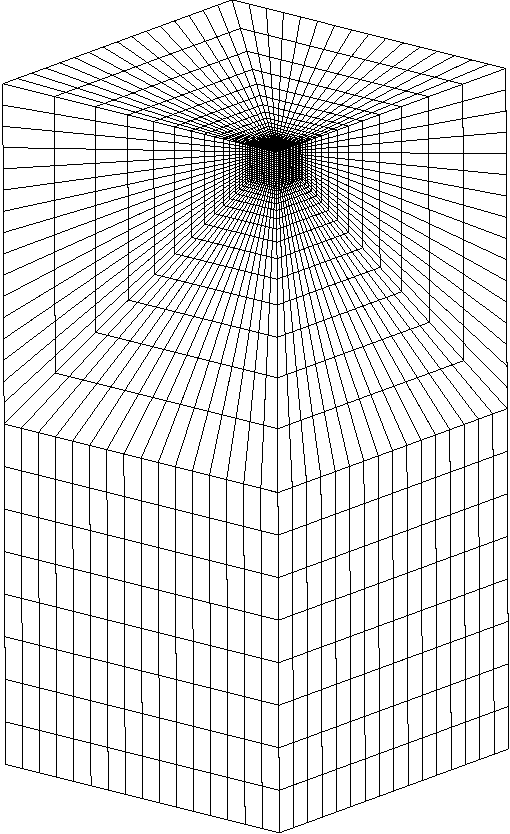
\includegraphics[height=0.3\textheight]{pictures/grid.png}
	\caption{ Сетка
	}
	\label{fig:grid}
\end{figure}
\begin{figure}[h!]
	%\centering
	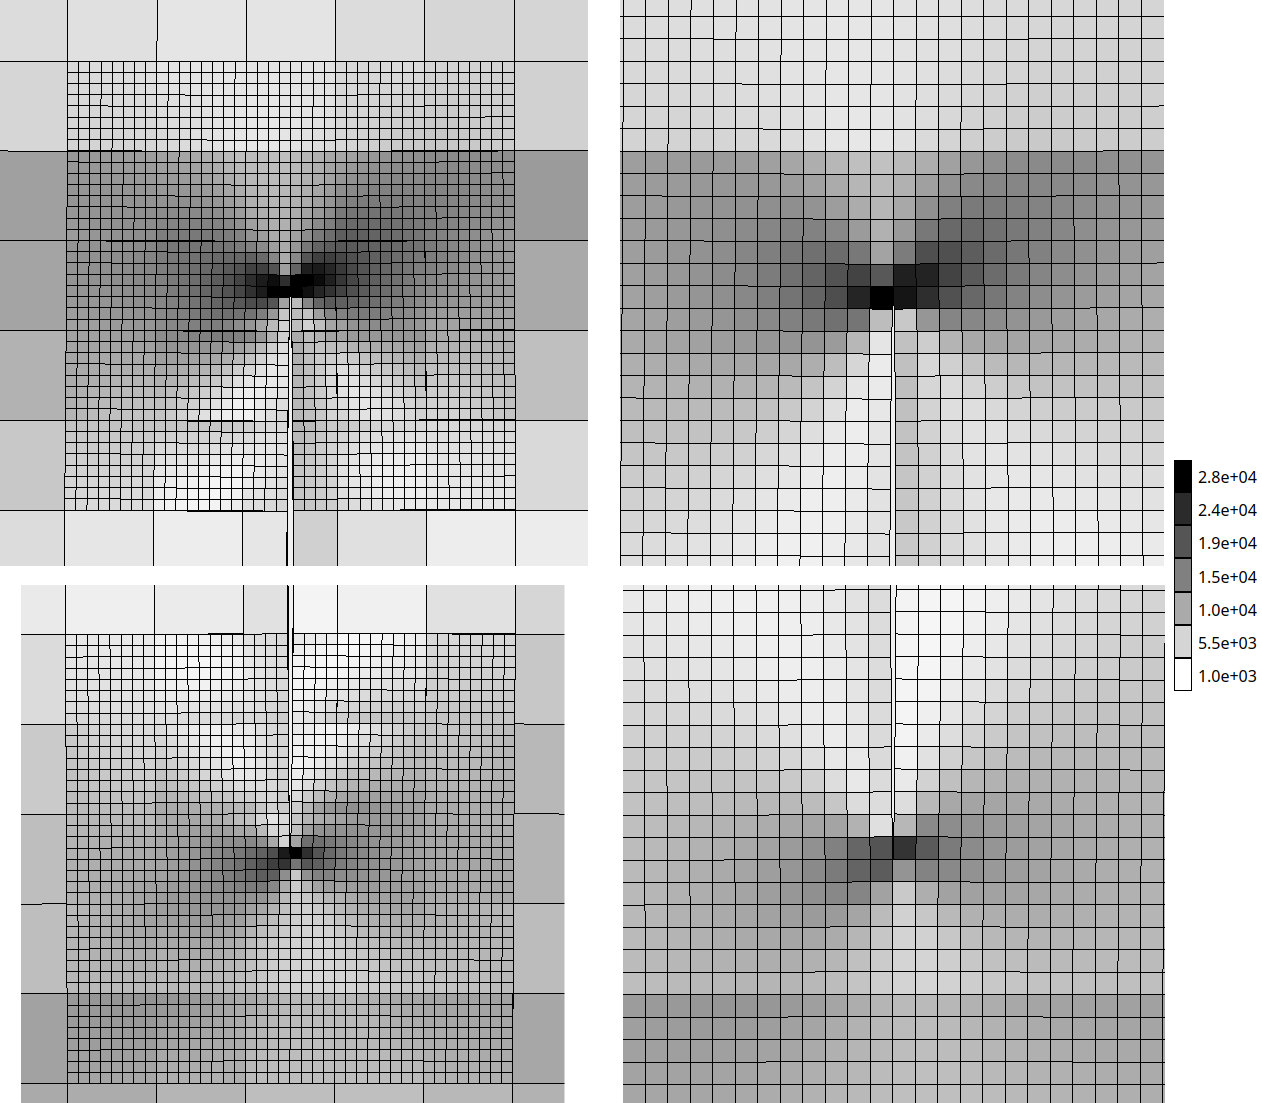
\includegraphics[height=0.4\textheight]{pictures/0.85_top_bot}
	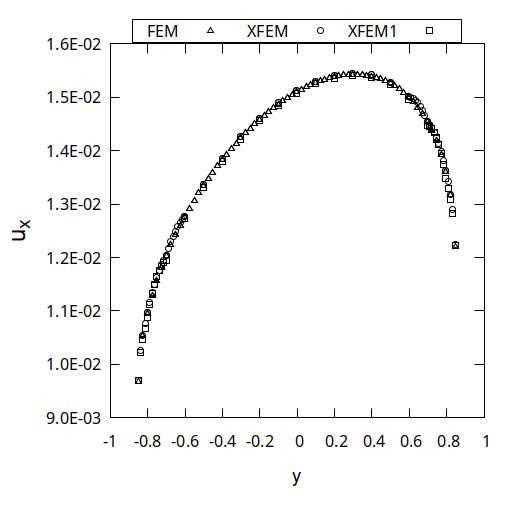
\includegraphics[height=0.4\textheight]{pictures/0.85_ux}
	\caption{ Трещина $-0.85<y<0.85$. Сверху показаны эквивалентные напряжения (слева XFEM, справа FEM). На графике показано сравнение перемещений по оси $x$ в правой части трещины. Напряжения в XFEM достигали значения $3.8\cdot 10^{4}$.
	}
	\label{fig:res1}
\end{figure}
\begin{figure}[h!]
	%\centering
	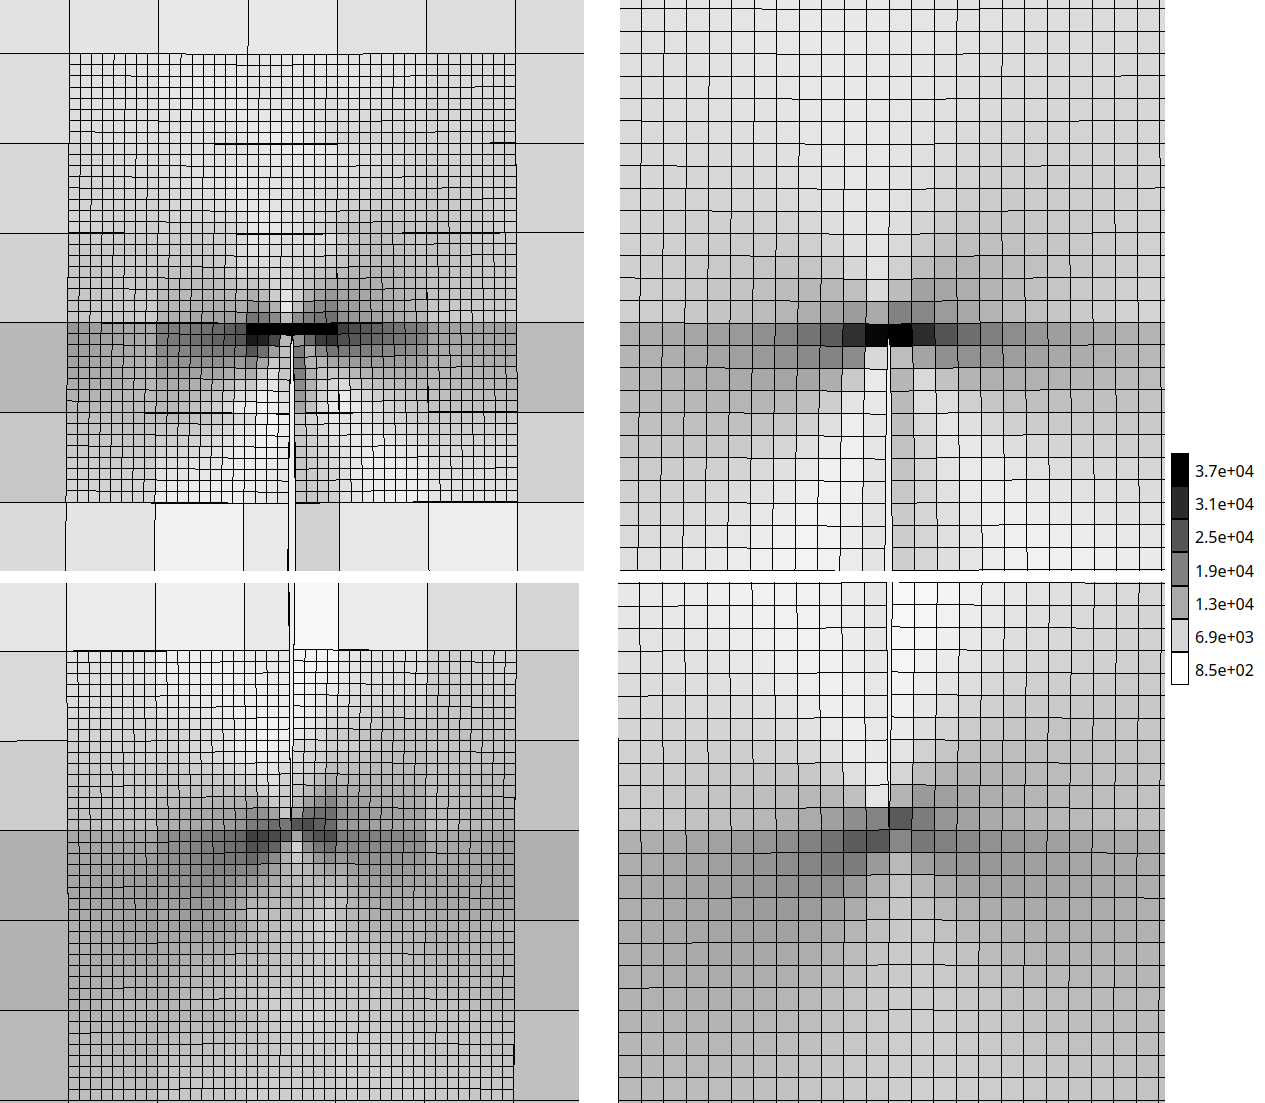
\includegraphics[height=0.4\textheight]{pictures/1.0_top_bot}
	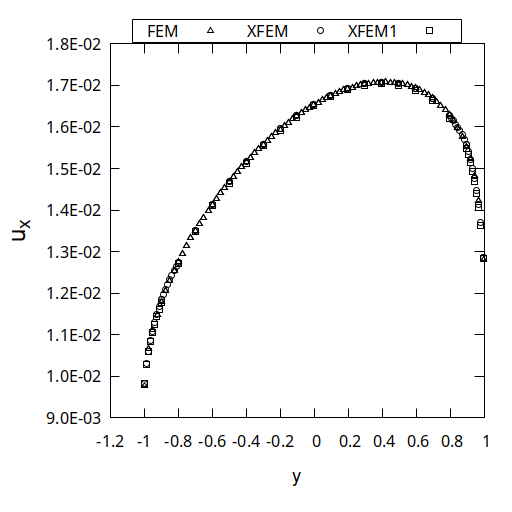
\includegraphics[height=0.4\textheight]{pictures/1.0_ux}
	\caption{ Трещина $-1<y<1$. Сверху показаны эквивалентные напряжения (слева XFEM, справа FEM). На графике показано сравнение перемещений по оси $x$ в правой части трещины. Напряжения в XFEM достигали значения $4.3\cdot 10^{4}$.
	}
	\label{fig:res2}
\end{figure}
\begin{figure}[h!]
	%\centering
	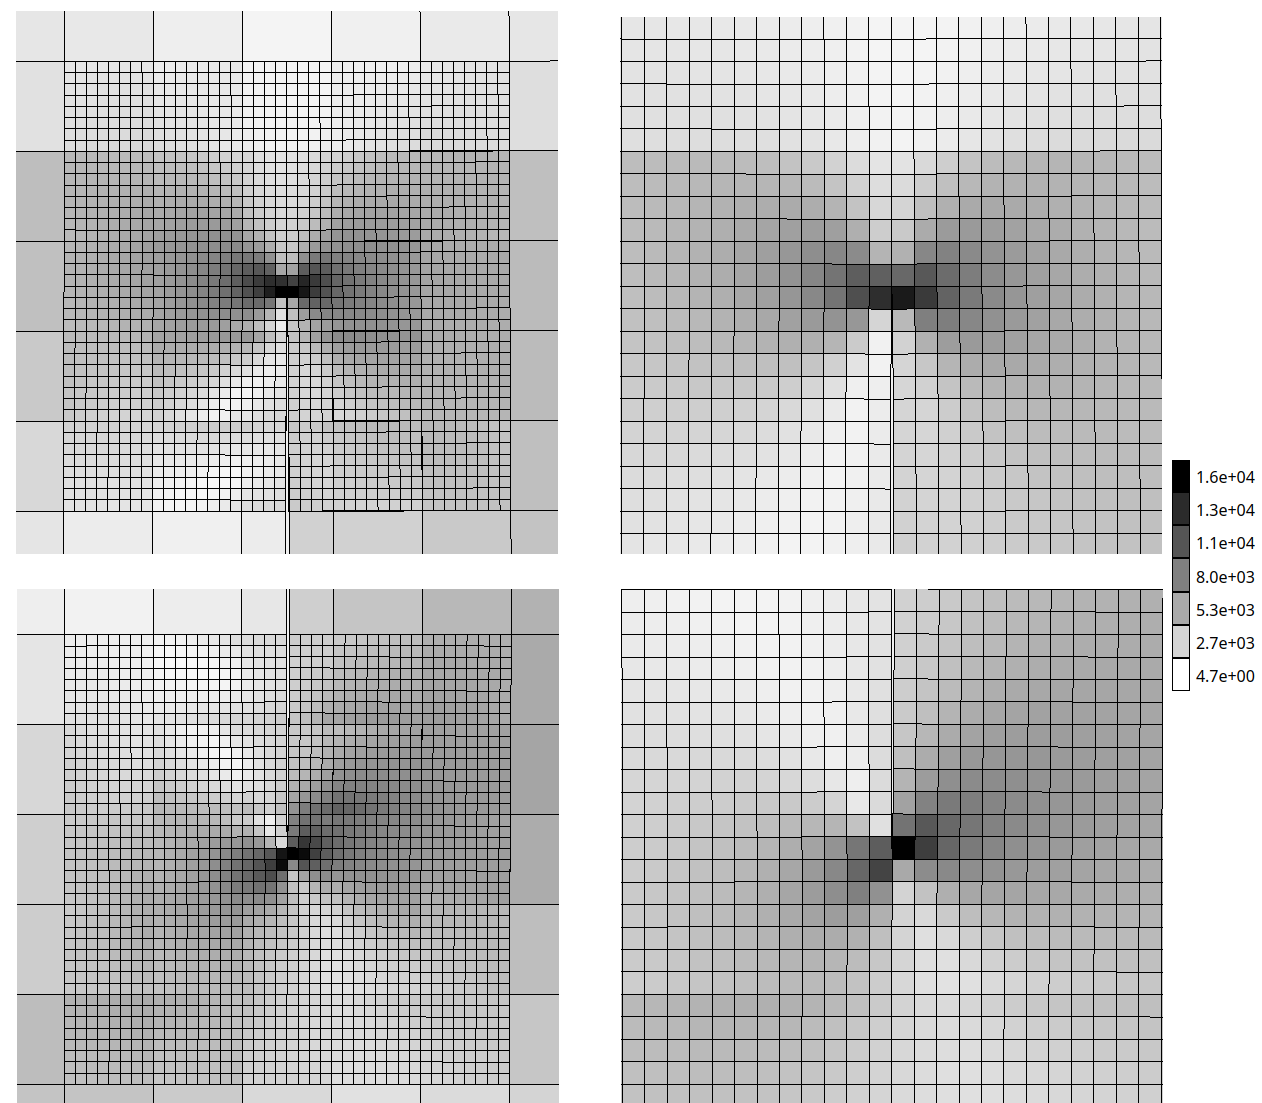
\includegraphics[height=0.4\textheight]{pictures/bc2_0.85_top_bot}
	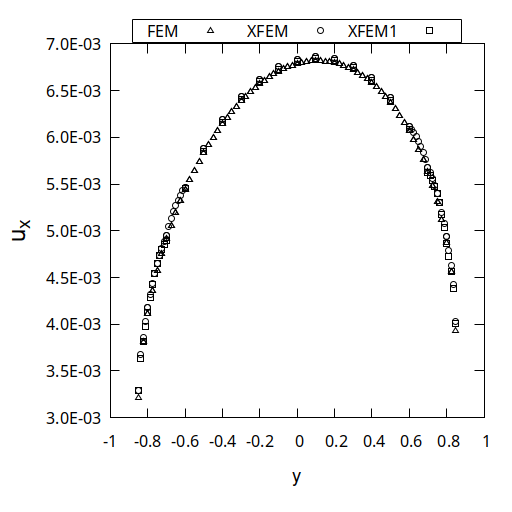
\includegraphics[height=0.4\textheight]{pictures/bc2_0.85_ux}
	\caption{ Трещина $-0.85<y<0.85$, давление приложено к правой части трещины. Сверху показаны эквивалентные напряжения (слева XFEM, справа FEM). На графике показано сравнение перемещений по оси $x$ в правой части трещины. Напряжения в XFEM достигали значения $2.0\cdot 10^{4}$.
	}
	\label{fig:res3}
\end{figure}

%%% Local Variables:
%%% mode: latex
%%% TeX-master: "rpz"
%%% End:


% \iffalse
% \include{20-analysis}
% \fi

 
% \include{30-design}
% \include{40-impl}
% \include{50-research}
% \include{60-economics}
% \include{70-bzd}

\backmatter %% Здесь заканчивается нумерованная часть документа и начинаются ссылки и
            
% \include{80-conclusion}%% заключение




\appendix   % Тут идут приложения

% \include{90-appendix1}

% \include{91-appendix2}


%\fi

\end{document}

%%% Local Variables:
%%% mode: latex
%%% TeX-master: t
%%% End:
